\documentclass[11pt]{article}

\usepackage[margin=1in]{geometry}
\usepackage{amsmath,amssymb}
\usepackage{xcolor}
\usepackage{tikz}
\usetikzlibrary{arrows.meta,positioning,calc,fit,backgrounds,decorations.pathreplacing}
\usepackage{booktabs}
\usepackage{listings}
\usepackage{enumitem}
\usepackage{caption}
\usepackage{hyperref}
\hypersetup{colorlinks=true,linkcolor=RankA,citecolor=RankA,urlcolor=RankC}

% ---- rank colours (colour-blind friendly-ish) ----
\definecolor{RankA}{RGB}{31,119,180}
\definecolor{RankB}{RGB}{214,39,40}
\definecolor{RankC}{RGB}{44,160,44}
\definecolor{RankD}{RGB}{148,103,189}
\definecolor{ink}{RGB}{25,28,35}
\definecolor{soft}{RGB}{120,128,140}

\newcommand{\rk}[1]{\textcolor{RankA}{#1}}
\newcommand{\dv}{\,\mathrm{d}v\,}
\newcommand{\Herm}{^{\mathsf{H}}}
\newcommand{\Ngrid}{N_{\mathrm{grid}}}
\newcommand{\Rank}{\mathtt{rank}}

\lstset{
  basicstyle=\ttfamily\small,
  keywordstyle=\color{RankA}\bfseries,
  commentstyle=\color{soft}\itshape,
  columns=fullflexible,
  breaklines=true,
  showstringspaces=false,
  language=C,
}

\title{\vspace{-1.2cm}\bfseries Distributed Parallelization of Orthogonalization\\ and Diagonalization in \texttt{filter\_mpi}}
\author{FilterBSE --- MPI ring / Gram-matrix implementation}
\date{\today}

\begin{document}
\maketitle
\vspace{-0.6cm}

\begin{abstract}
\noindent
The filter-diagonalization pipeline has three stages: \textbf{(1)~Filter},
\textbf{(2)~Orthogonalize}, and \textbf{(3)~Diagonalize}. Stage~1 is
embarrassingly parallel and already MPI-distributed. This note documents the
new distributed implementations of stages~2 and~3 (\texttt{dist\_linalg.c}),
which keep the filtered states \emph{column-distributed} across MPI ranks --
never gathering the full $\Ngrid\!\times\!N$ state matrix onto a single node --
and reduce every large operation to (i)~local BLAS-3 products and
(ii)~communication of only tiny $N\!\times\!N$ matrices. No ScaLAPACK is
required. The orthogonalization is a distributed \emph{singular value
decomposition via the Gram matrix}; the diagonalization distributes the basis
transformations (``integrals'') that dominate its cost.
\end{abstract}

\section{Data layout: column (cyclic-block) distribution}

Let the matrix of filtered states be
\[
  A \;=\; \big[\,a_0\ \ a_1\ \ \cdots\ \ a_{N-1}\,\big]\;\in\;\mathbb{C}^{M\times N},
  \qquad M=\Ngrid \sim 10^{8},\quad N \sim 10^{3},
\]
where each \emph{column} $a_i\in\mathbb{C}^{M}$ is one full-grid wavefunction and
$M = \texttt{nspinngrid}$ is the (huge) number of grid degrees of freedom. The
matrix is extremely \emph{tall and skinny}. With $P$ MPI ranks, rank $p$ owns a
contiguous block of $n_p$ columns,
\[
  A_p \;=\; A[:,\,\mathcal{C}_p]\in\mathbb{C}^{M\times n_p},\qquad
  \mathcal{C}_p=[\,o_p,\,o_p+n_p\,),\qquad \sum_{p=0}^{P-1} n_p = N,
\]
so global state $g$ lives on rank $\lfloor g/n\rfloor$ (uniform $n_p=n$ out of
the filter). This is exactly the distribution the Filter stage produces, and
exactly what the Hamiltonian application needs (each FFT-based $\hat H|\psi\rangle$
requires one \emph{whole} state on one rank). It is preserved throughout.

\begin{figure}[h]
\centering
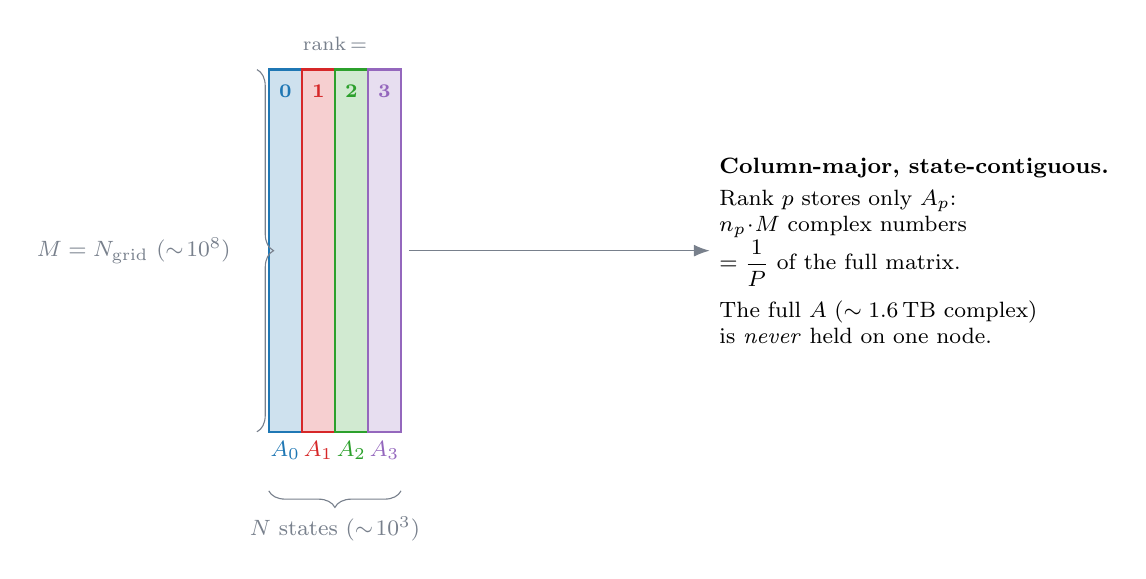
\begin{tikzpicture}[scale=1.0]
  % tall-skinny matrix A, columns coloured by owning rank
  \def\H{4.6}    % matrix height
  \def\cw{0.42}  % column-block width
  \foreach \i/\col in {0/RankA,1/RankB,2/RankC,3/RankD}{
    \fill[\col!22] ({\i*\cw},0) rectangle ({(\i+1)*\cw},\H);
    \draw[\col,thick] ({\i*\cw},0) rectangle ({(\i+1)*\cw},\H);
    \node[below,\col] at ({(\i+0.5)*\cw},0) {\footnotesize $A_{\i}$};
    \node[\col,font=\scriptsize\bfseries] at ({(\i+0.5)*\cw},{\H-0.28}) {\i};
  }
  \node[above,soft,font=\scriptsize] at (2*\cw,{\H+0.12}) {rank\,=};
  % brace for M rows
  \draw[decorate,decoration={brace,amplitude=6pt},soft]
        (-0.15,\H) -- (-0.15,0) node[midway,left=6pt,soft]{\footnotesize $M=\Ngrid\ (\sim\!10^{8})$};
  % brace for N cols
  \draw[decorate,decoration={brace,amplitude=6pt,mirror},soft]
        (0,-0.75) -- ({4*\cw},-0.75) node[midway,below=6pt,soft]{\footnotesize $N$ states $(\sim\!10^{3})$};

  % arrow to storage note
  \node[right=2.4cm of {(4*\cw,\H/2)},align=left,font=\footnotesize] (note)
    at (3.2,\H/2)
    {\textbf{Column-major, state-contiguous.}\\[2pt]
     Rank $p$ stores only $A_p$:\\
     $n_p\!\cdot\! M$ complex numbers\\
     $=\dfrac{1}{P}$ of the full matrix.\\[4pt]
     The full $A$ ($\sim 1.6$\,TB complex)\\
     is \emph{never} held on one node.};
  \draw[-{Latex[length=2mm]},soft] ({4*\cw+0.1},\H/2) -- (note.west);
\end{tikzpicture}
\caption{Column-block distribution of the tall-skinny state matrix $A$. Each
rank owns whole columns (states), full grid length each.}
\label{fig:layout}
\end{figure}

The physical inner product carries the grid volume element $\dv=\mathrm{d}x\,\mathrm{d}y\,\mathrm{d}z$:
\begin{equation}
  \langle x,\,y\rangle \;=\; \dv\sum_{g=0}^{M-1} \overline{x_g}\,y_g,
  \qquad\text{so}\qquad
  S \;=\; \dv\,A\Herm A \in\mathbb{C}^{N\times N},\quad
  S_{ij}=\langle a_i,\,a_j\rangle .
  \label{eq:gram}
\end{equation}

\section{The two ring primitives}

Both stages reduce to two operations on column-distributed data. Each is
realised by circulating the large column blocks once around the rank ring
(\autoref{fig:ring}), doing a local $\mathtt{zgemm}$ at every hop, while only
tiny $N\!\times\!N$ data is ever reduced.

\paragraph{(P1) Distributed Gram / overlap matrix.}
$S=\dv\,A\Herm B$ with $A,B$ identically column-distributed. Rank $p$ holds its
panel $B_p$ \emph{fixed} and receives every $A_q$ in turn; the local product
\begin{equation}
  S[\mathcal{C}_q,\mathcal{C}_p] \;=\; \dv\,A_q\Herm B_p \;\in\;\mathbb{C}^{n_q\times n_p}
  \qquad(\text{one }\mathtt{zgemm},\ \text{contraction over the }M\text{ rows})
  \label{eq:panel}
\end{equation}
fills the column panel $S[:,\mathcal{C}_p]$. After $P$ hops an
\texttt{MPI\_Allgatherv} of the panels assembles the full $S$ on every rank.
For orthogonalization $B=A$; for diagonalization $B=\hat H U$.

\paragraph{(P2) Distributed back-transform.}
$\mathrm{out}=A\,W$ with $W\in\mathbb{C}^{N\times r}$ small and replicated. Rank
$p$ accumulates its output columns $\mathrm{out}[:,\mathcal{K}_p]$ by receiving
each $A_q$ and adding
\begin{equation}
  \mathrm{out}[:,\mathcal{K}_p] \;\mathrel{+}=\; A_q\, W[\mathcal{C}_q,\mathcal{K}_p]
  \qquad(\text{one accumulating }\mathtt{zgemm}\ \text{per hop}).
  \label{eq:back}
\end{equation}
The output is left column-distributed, ready for the next stage.

\begin{figure}[h]
\centering
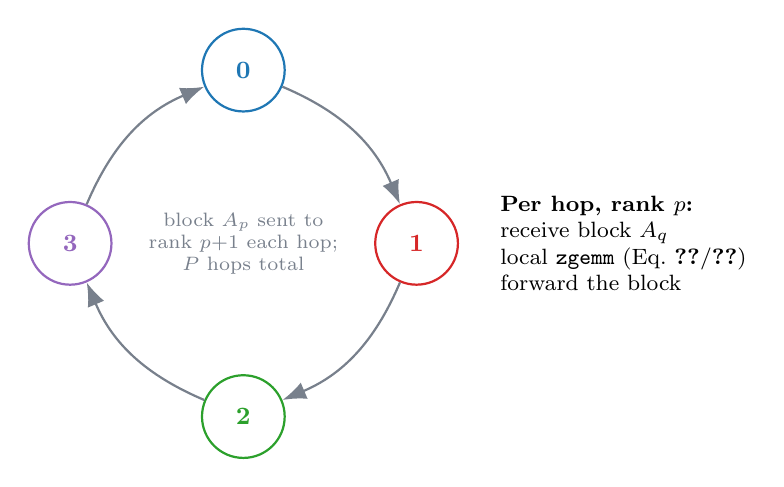
\begin{tikzpicture}[scale=1.0,
   ranknode/.style={circle,draw,thick,minimum size=1.05cm,font=\small\bfseries}]
  \node[ranknode,RankA] (r0) at (90:2.2)  {0};
  \node[ranknode,RankB] (r1) at (0:2.2)   {1};
  \node[ranknode,RankC] (r2) at (-90:2.2) {2};
  \node[ranknode,RankD] (r3) at (180:2.2) {3};
  \foreach \a/\b in {r0/r1,r1/r2,r2/r3,r3/r0}{
    \draw[-{Latex[length=3mm]},thick,soft] (\a) to[bend left=22] (\b);
  }
  \node[align=center,font=\scriptsize,soft] at (0,0)
     {block $A_p$ sent to\\ rank $p{+}1$ each hop;\\ $P$ hops total};
  % side legend
  \node[right=0.4cm of r1,align=left,font=\footnotesize] {%
    \textbf{Per hop, rank $p$:}\\
    receive block $A_{q}$\\
    local $\mathtt{zgemm}$ (Eq.~\ref{eq:panel}/\ref{eq:back})\\
    forward the block};
\end{tikzpicture}
\caption{Ring communication. The large column blocks circulate once
($P{-}1$ neighbour exchanges via \texttt{MPI\_Sendrecv\_replace}); total data
moved $=O(MN)$, i.e.\ the full matrix once, independent of $P$. Local flops per
primitive are $O(MN^2/P)$.}
\label{fig:ring}
\end{figure}

\begin{figure}[h]
\centering
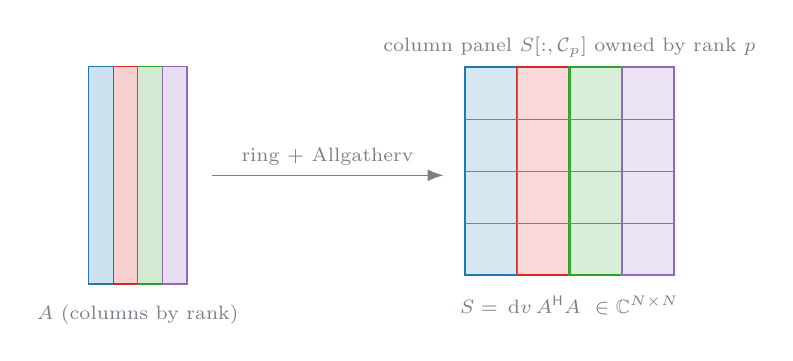
\begin{tikzpicture}[scale=0.92]
  % local blocks A_q (left), tall skinny
  \def\H{3.0}\def\cw{0.34}
  \begin{scope}[shift={(0,0)}]
    \foreach \i/\col in {0/RankA,1/RankB,2/RankC,3/RankD}{
      \fill[\col!22]({\i*\cw},0) rectangle ({(\i+1)*\cw},\H);
      \draw[\col]({\i*\cw},0) rectangle ({(\i+1)*\cw},\H);
    }
    \node[below,soft,font=\scriptsize] at (2*\cw,-0.15){$A$ (columns by rank)};
  \end{scope}
  % the N x N gram, filled panel-by-panel
  \begin{scope}[shift={(5.2,0)}]
    \def\g{0.72}
    \foreach \c/\col in {0/RankA,1/RankB,2/RankC,3/RankD}{
       \fill[\col!18] ({\c*\g},{\H-4*\g}) rectangle ({(\c+1)*\g},\H);
       \draw[\col,thick] ({\c*\g},{\H-4*\g}) rectangle ({(\c+1)*\g},\H);
       \node[above,\col,font=\scriptsize] at ({(\c+0.5)*\g},\H){\,};
    }
    % grid lines
    \foreach \k in {1,2,3}{
      \draw[soft,very thin] ({\k*\g},{\H-4*\g}) -- ({\k*\g},\H);
      \draw[soft,very thin] (0,{\H-\k*\g}) -- ({4*\g},{\H-\k*\g});
    }
    \node[below,soft,font=\scriptsize] at (2*\g,{\H-4*\g-0.15}){$S=\dv A\Herm A\ \in\mathbb{C}^{N\times N}$};
    \node[above,soft,font=\scriptsize] at (2*\g,\H){column panel $S[:,\mathcal C_p]$ owned by rank $p$};
  \end{scope}
  \draw[-{Latex[length=2mm]},soft] (1.7,\H/2) -- (4.9,\H/2)
     node[midway,above,font=\scriptsize,soft]{ring + Allgatherv};
\end{tikzpicture}
\caption{Primitive P1: each rank builds one \emph{column panel} of the small
$N\!\times\!N$ Gram matrix from local products (Eq.~\ref{eq:panel}); an
\texttt{Allgatherv} yields the full $S$ (Hermitian) on every rank.}
\label{fig:gram}
\end{figure}

\section{Stage 2 --- Distributed orthogonalization (SVD via the Gram matrix)}

We want an orthonormal basis of the filtered states, discarding numerically
redundant directions using the singular-value threshold \texttt{SVDEPS}. For an
$M\gg N$ matrix, forming the Gram matrix and diagonalizing it is the standard
tall-skinny SVD and maps perfectly onto the column layout.

\paragraph{Step 1 --- Gram matrix (P1).} Equation~\eqref{eq:gram}, formed by the
ring. Because $A\Herm A = V\Lambda V\Herm$ shares its right singular vectors and
squared singular values with the SVD $A=U_{\!A}\Sigma V\Herm$, one small
Hermitian eigensolve gives the full spectral information:
\begin{equation}
  S \;=\; V\,\Lambda\,V\Herm,\qquad
  \Lambda=\operatorname{diag}(\lambda_1\ge\cdots\ge\lambda_N\ge 0),\qquad
  \sigma_i=\sqrt{\lambda_i}.
  \label{eq:eig}
\end{equation}
This $N\!\times\!N$ eigenproblem is solved with LAPACK \texttt{zheev} on the
root and broadcast (so every rank is bit-identical).

\paragraph{Step 2 --- Rank / cutoff.} Retain the leading $r$ directions,
\begin{equation}
  r \;=\; \#\Big\{\, i : \frac{\sigma_i}{\sigma_1}\ \ge\ \varepsilon \,\Big\},
  \qquad
  \varepsilon=\max\!\big(\texttt{SVDEPS},\ \varepsilon_{\mathrm{floor}}\big),
  \qquad
  \varepsilon_{\mathrm{floor}}=10^{-7}.
  \label{eq:cutoff}
\end{equation}
The floor is essential: a Gram (normal-equations) method squares the condition
number, so it cannot resolve singular values below
$\sqrt{\varepsilon_{\mathrm{mach}}}\approx1.5\times10^{-8}$ relative to
$\sigma_1$ -- below that the squared spectrum $\lambda_i=\sigma_i^2$ sinks under
the eigensolver noise floor. Clamping $\varepsilon$ to $10^{-7}$ guarantees that
retained directions are genuine, not noise. (A finer cutoff at scale would
require a QR-based TSQR instead of the Gram matrix.)

\paragraph{Step 3 --- Orthonormal basis (P2).} Build the small back-transform
matrix and apply it via the ring:
\begin{equation}
  W \;=\; V_r\,\Lambda_r^{-1/2}\ \in\ \mathbb{C}^{N\times r},
  \qquad
  U \;=\; A\,W \;=\; A\,V_r\,\Lambda_r^{-1/2},
  \label{eq:U}
\end{equation}
where $V_r,\Lambda_r$ keep the leading $r$ columns/values. The columns of $U$
are orthonormal in the weighted inner product:
\begin{align}
  \langle U,U\rangle
  &= \dv\,U\Herm U
   = \Lambda_r^{-1/2} V_r\Herm \big(\dv\,A\Herm A\big) V_r \Lambda_r^{-1/2}
   = \Lambda_r^{-1/2} V_r\Herm S\, V_r \Lambda_r^{-1/2} \notag\\
  &= \Lambda_r^{-1/2}\,\Lambda_r\,\Lambda_r^{-1/2} \;=\; I_r .
  \label{eq:orthoproof}
\end{align}

\paragraph{Step 4 --- Second pass (polish).} To remove the residual
non-orthonormality that the squared conditioning leaves in the tail, the whole
procedure is repeated once with $A\leftarrow U$ (a CholeskyQR2-style refinement).
The second Gram is $\approx I_r$, so it does not truncate further but restores
$\langle U,U\rangle=I_r$ to machine precision:
\[
  \boxed{\;U^{(2)} = U^{(1)} V_r^{(2)} \big(\Lambda_r^{(2)}\big)^{-1/2},\qquad
  \big\| \dv\,U^{(2)\mathsf H} U^{(2)} - I_r\big\|_{\max}\lesssim 10^{-15}. \;}
\]

\medskip
The output $U\in\mathbb{C}^{M\times r}$ is column-distributed over a fresh block
partition $\mathcal K_p$ of the $r$ retained states.

\section{Stage 3 --- Distributed diagonalization}

The eigenvectors are computed in the small orthonormal basis $U$ and transformed
back to the grid. Every large operation is again local + one small reduction.

\paragraph{Step 1 --- Apply the Hamiltonian (local).} Each rank applies $\hat H$
(kinetic via FFT, local potential, non-local/spin--orbit projectors) to \emph{its
own} states -- embarrassingly parallel, reusing \texttt{p\_hamiltonian}:
\[
  (\hat H U)_p \;=\; \hat H\,U_p,\qquad k\in\mathcal K_p .
\]

\paragraph{Step 2 --- Reduced Hamiltonian (P1).} Form the $r\!\times\!r$ matrix
with the Gram primitive using $B=\hat H U$:
\begin{equation}
  \widetilde H \;=\; \dv\,U\Herm \hat H\,U \ \in\ \mathbb{C}^{r\times r},
  \qquad \widetilde H_{ij}=\langle u_i,\hat H u_j\rangle,\qquad
  \widetilde H = \widetilde H\Herm .
  \label{eq:Hred}
\end{equation}

\paragraph{Step 3 --- Small eigenproblem.} On the root, then broadcast:
\begin{equation}
  \widetilde H \;=\; C\,E\,C\Herm,\qquad
  E=\operatorname{diag}(E_1\le\cdots\le E_r),
  \label{eq:smalleig}
\end{equation}
so $E$ are the quasiparticle energies and $C\in\mathbb{C}^{r\times r}$ the
eigenvectors in the filtered basis.

\paragraph{Step 4 --- Back to the grid basis (P2).}
\begin{equation}
  \Psi \;=\; U\,C,\qquad \psi_k=\sum_{i=1}^{r} u_i\,C_{ik},
  \label{eq:psigrid}
\end{equation}
again a ring back-transform, leaving $\Psi$ column-distributed.

\paragraph{Step 5 --- Eigenvalue variance (local).} The ghost-state diagnostic is
purely local because each rank owns whole states. Using Hermiticity,
$\langle\psi|\hat H^2|\psi\rangle=\|\hat H\psi\|^2$, so a \emph{single} extra
Hamiltonian application suffices:
\begin{equation}
  \sigma_{E,k}^2
  \;=\; \langle\psi_k|\hat H^2|\psi_k\rangle - \langle\psi_k|\hat H|\psi_k\rangle^2
  \;=\; \big\|\hat H\psi_k\big\|^2 - E_k^2 .
  \label{eq:sigma}
\end{equation}

\paragraph{Output.} Eigenvectors are written to \texttt{psi.dat} with collective
MPI-IO: state $g$ is placed at byte offset
$g\cdot\texttt{stlen}\cdot 8$ with $\texttt{stlen}=\texttt{complex\_idx}\cdot M$,
matching the serial writer and the \texttt{get\_n\_states.x}/BSE readers. Each
rank writes its block $\mathcal K_p$ directly at its global offset; energies and
$\sigma_E$ are gathered to the root for \texttt{eval.dat}.

\section{Cost and communication}

\begin{center}
\renewcommand{\arraystretch}{1.25}
\begin{tabular}{@{}lccc@{}}
\toprule
Operation & Local flops & Communication & Reduced size \\
\midrule
Gram $S=\dv A\Herm A$ (P1)        & $O(MN^2/P)$ & $O(MN)$ ring + Allgatherv & $N\!\times\!N$ \\
Back-transform $A\,W$ (P2)         & $O(MNr/P)$  & $O(MN)$ ring              & --- \\
Small eigensolve (\texttt{zheev})  & $O(N^3)$ (root) & Bcast $N\!\times\!N$  & $N\!\times\!N$ \\
$\hat H U$ (per state)             & $O(\tfrac{N}{P} M\log M)$ & none          & --- \\
\bottomrule
\end{tabular}
\end{center}

Because $N\!\sim\!10^{3}$, the $O(MN^2)$ compute dominates the $O(MN)$
communication by a factor $\sim N$: the ring exchanges are cheap relative to the
GEMMs, and no operation ever materialises more than $O(MN/P)$ (one rank's share)
of the large data. Memory per rank stays at a small multiple of $A_p$.

\section{Validation}

\begin{center}
\renewcommand{\arraystretch}{1.25}
\begin{tabular}{@{}lll@{}}
\toprule
Test & Metric & Result \\
\midrule
Unit: ring Gram vs.\ dense (4 ranks)          & $\max|S_{\text{ring}}-S_{\text{ref}}|$ & $1.6\times10^{-13}$ \\
Unit: distributed SVD, rank-deficient         & retained rank $r$ & correct (uneven split) \\
Unit: orthonormality                          & $\max|\dv\,U\Herm U-I|$ & $2.4\times10^{-15}$ \\
End-to-end CsPbI$_3$ (4 ranks) vs.\ serial    & converged eigenvalues & match to $1.6\times10^{-6}$\,eV \\
End-to-end: \texttt{psi.dat}                   & byte layout / offsets & exact \\
\bottomrule
\end{tabular}
\end{center}

\noindent
The distributed path retains slightly fewer states than the serial
$\texttt{SVDEPS}=10^{-10}$ SVD (the tail trimmed by the $10^{-7}$ Gram floor of
Eq.~\ref{eq:cutoff}); those are the ill-conditioned directions the $\sigma_E$
ghost filter removes anyway, and all converged physical eigenvalues agree with
the serial reference to $\sim\!10^{-6}$\,eV.

\end{document}
